% Options for packages loaded elsewhere
\PassOptionsToPackage{unicode}{hyperref}
\PassOptionsToPackage{hyphens}{url}
%
\documentclass[
]{article}
\usepackage{amsmath,amssymb}
\usepackage{lmodern}
\usepackage{iftex}
\ifPDFTeX
  \usepackage[T1]{fontenc}
  \usepackage[utf8]{inputenc}
  \usepackage{textcomp} % provide euro and other symbols
\else % if luatex or xetex
  \usepackage{unicode-math}
  \defaultfontfeatures{Scale=MatchLowercase}
  \defaultfontfeatures[\rmfamily]{Ligatures=TeX,Scale=1}
\fi
% Use upquote if available, for straight quotes in verbatim environments
\IfFileExists{upquote.sty}{\usepackage{upquote}}{}
\IfFileExists{microtype.sty}{% use microtype if available
  \usepackage[]{microtype}
  \UseMicrotypeSet[protrusion]{basicmath} % disable protrusion for tt fonts
}{}
\makeatletter
\@ifundefined{KOMAClassName}{% if non-KOMA class
  \IfFileExists{parskip.sty}{%
    \usepackage{parskip}
  }{% else
    \setlength{\parindent}{0pt}
    \setlength{\parskip}{6pt plus 2pt minus 1pt}}
}{% if KOMA class
  \KOMAoptions{parskip=half}}
\makeatother
\usepackage{xcolor}
\IfFileExists{xurl.sty}{\usepackage{xurl}}{} % add URL line breaks if available
\IfFileExists{bookmark.sty}{\usepackage{bookmark}}{\usepackage{hyperref}}
\hypersetup{
  pdftitle={R Notebook},
  hidelinks,
  pdfcreator={LaTeX via pandoc}}
\urlstyle{same} % disable monospaced font for URLs
\usepackage[margin=1in]{geometry}
\usepackage{color}
\usepackage{fancyvrb}
\newcommand{\VerbBar}{|}
\newcommand{\VERB}{\Verb[commandchars=\\\{\}]}
\DefineVerbatimEnvironment{Highlighting}{Verbatim}{commandchars=\\\{\}}
% Add ',fontsize=\small' for more characters per line
\usepackage{framed}
\definecolor{shadecolor}{RGB}{248,248,248}
\newenvironment{Shaded}{\begin{snugshade}}{\end{snugshade}}
\newcommand{\AlertTok}[1]{\textcolor[rgb]{0.94,0.16,0.16}{#1}}
\newcommand{\AnnotationTok}[1]{\textcolor[rgb]{0.56,0.35,0.01}{\textbf{\textit{#1}}}}
\newcommand{\AttributeTok}[1]{\textcolor[rgb]{0.77,0.63,0.00}{#1}}
\newcommand{\BaseNTok}[1]{\textcolor[rgb]{0.00,0.00,0.81}{#1}}
\newcommand{\BuiltInTok}[1]{#1}
\newcommand{\CharTok}[1]{\textcolor[rgb]{0.31,0.60,0.02}{#1}}
\newcommand{\CommentTok}[1]{\textcolor[rgb]{0.56,0.35,0.01}{\textit{#1}}}
\newcommand{\CommentVarTok}[1]{\textcolor[rgb]{0.56,0.35,0.01}{\textbf{\textit{#1}}}}
\newcommand{\ConstantTok}[1]{\textcolor[rgb]{0.00,0.00,0.00}{#1}}
\newcommand{\ControlFlowTok}[1]{\textcolor[rgb]{0.13,0.29,0.53}{\textbf{#1}}}
\newcommand{\DataTypeTok}[1]{\textcolor[rgb]{0.13,0.29,0.53}{#1}}
\newcommand{\DecValTok}[1]{\textcolor[rgb]{0.00,0.00,0.81}{#1}}
\newcommand{\DocumentationTok}[1]{\textcolor[rgb]{0.56,0.35,0.01}{\textbf{\textit{#1}}}}
\newcommand{\ErrorTok}[1]{\textcolor[rgb]{0.64,0.00,0.00}{\textbf{#1}}}
\newcommand{\ExtensionTok}[1]{#1}
\newcommand{\FloatTok}[1]{\textcolor[rgb]{0.00,0.00,0.81}{#1}}
\newcommand{\FunctionTok}[1]{\textcolor[rgb]{0.00,0.00,0.00}{#1}}
\newcommand{\ImportTok}[1]{#1}
\newcommand{\InformationTok}[1]{\textcolor[rgb]{0.56,0.35,0.01}{\textbf{\textit{#1}}}}
\newcommand{\KeywordTok}[1]{\textcolor[rgb]{0.13,0.29,0.53}{\textbf{#1}}}
\newcommand{\NormalTok}[1]{#1}
\newcommand{\OperatorTok}[1]{\textcolor[rgb]{0.81,0.36,0.00}{\textbf{#1}}}
\newcommand{\OtherTok}[1]{\textcolor[rgb]{0.56,0.35,0.01}{#1}}
\newcommand{\PreprocessorTok}[1]{\textcolor[rgb]{0.56,0.35,0.01}{\textit{#1}}}
\newcommand{\RegionMarkerTok}[1]{#1}
\newcommand{\SpecialCharTok}[1]{\textcolor[rgb]{0.00,0.00,0.00}{#1}}
\newcommand{\SpecialStringTok}[1]{\textcolor[rgb]{0.31,0.60,0.02}{#1}}
\newcommand{\StringTok}[1]{\textcolor[rgb]{0.31,0.60,0.02}{#1}}
\newcommand{\VariableTok}[1]{\textcolor[rgb]{0.00,0.00,0.00}{#1}}
\newcommand{\VerbatimStringTok}[1]{\textcolor[rgb]{0.31,0.60,0.02}{#1}}
\newcommand{\WarningTok}[1]{\textcolor[rgb]{0.56,0.35,0.01}{\textbf{\textit{#1}}}}
\usepackage{graphicx}
\makeatletter
\def\maxwidth{\ifdim\Gin@nat@width>\linewidth\linewidth\else\Gin@nat@width\fi}
\def\maxheight{\ifdim\Gin@nat@height>\textheight\textheight\else\Gin@nat@height\fi}
\makeatother
% Scale images if necessary, so that they will not overflow the page
% margins by default, and it is still possible to overwrite the defaults
% using explicit options in \includegraphics[width, height, ...]{}
\setkeys{Gin}{width=\maxwidth,height=\maxheight,keepaspectratio}
% Set default figure placement to htbp
\makeatletter
\def\fps@figure{htbp}
\makeatother
\setlength{\emergencystretch}{3em} % prevent overfull lines
\providecommand{\tightlist}{%
  \setlength{\itemsep}{0pt}\setlength{\parskip}{0pt}}
\setcounter{secnumdepth}{-\maxdimen} % remove section numbering
\ifLuaTeX
  \usepackage{selnolig}  % disable illegal ligatures
\fi

\title{R Notebook}
\author{}
\date{\vspace{-2.5em}}

\begin{document}
\maketitle

\begin{Shaded}
\begin{Highlighting}[]
\NormalTok{cars }\OtherTok{=} \FunctionTok{c}\NormalTok{(}\DecValTok{1}\NormalTok{,}\DecValTok{3}\NormalTok{,}\DecValTok{6}\NormalTok{,}\DecValTok{4}\NormalTok{,}\DecValTok{9}\NormalTok{)}
\FunctionTok{plot}\NormalTok{(cars, }\AttributeTok{type=}\StringTok{\textquotesingle{}o\textquotesingle{}}\NormalTok{, }\AttributeTok{col=}\StringTok{\textquotesingle{}blue\textquotesingle{}}\NormalTok{)}
\FunctionTok{title}\NormalTok{(}\AttributeTok{main=}\StringTok{\textquotesingle{}Autos\textquotesingle{}}\NormalTok{, }\AttributeTok{col.main=}\StringTok{\textquotesingle{}red\textquotesingle{}}\NormalTok{, }\AttributeTok{font.main=}\DecValTok{4}\NormalTok{)}
\end{Highlighting}
\end{Shaded}

\includegraphics{17_1_21_files/figure-latex/unnamed-chunk-1-1.pdf}

\begin{Shaded}
\begin{Highlighting}[]
\NormalTok{cars   }\OtherTok{=} \FunctionTok{c}\NormalTok{(}\DecValTok{1}\NormalTok{,}\DecValTok{3}\NormalTok{,}\DecValTok{6}\NormalTok{,}\DecValTok{4}\NormalTok{,}\DecValTok{9}\NormalTok{)}
\NormalTok{trucks }\OtherTok{=} \FunctionTok{c}\NormalTok{(}\DecValTok{2}\NormalTok{,}\DecValTok{5}\NormalTok{,}\DecValTok{4}\NormalTok{,}\DecValTok{5}\NormalTok{,}\DecValTok{12}\NormalTok{)}

\CommentTok{\# Graph cars using a y axis that ranges from 0 to 12}
\FunctionTok{plot}\NormalTok{(cars, }\AttributeTok{type=}\StringTok{"o"}\NormalTok{, }\AttributeTok{col=}\StringTok{"blue"}\NormalTok{, }\AttributeTok{ylim=}\FunctionTok{c}\NormalTok{(}\DecValTok{0}\NormalTok{,}\DecValTok{12}\NormalTok{))}

\CommentTok{\# Graph trucks with red dashed line and square points}
\FunctionTok{lines}\NormalTok{(trucks, }\AttributeTok{type=}\StringTok{"o"}\NormalTok{, }\AttributeTok{pch=}\DecValTok{22}\NormalTok{, }\AttributeTok{lty=}\DecValTok{2}\NormalTok{, }\AttributeTok{col=}\StringTok{"red"}\NormalTok{)}

\CommentTok{\# Create a title with a red, bold/italic font}
\FunctionTok{title}\NormalTok{(}\AttributeTok{main=}\StringTok{"Autos"}\NormalTok{, }\AttributeTok{col.main=}\StringTok{"red"}\NormalTok{, }\AttributeTok{font.main=}\DecValTok{4}\NormalTok{)}
\end{Highlighting}
\end{Shaded}

\includegraphics{17_1_21_files/figure-latex/unnamed-chunk-2-1.pdf}

\begin{Shaded}
\begin{Highlighting}[]
\CommentTok{\# Define 2 vectors}
\NormalTok{cars }\OtherTok{\textless{}{-}} \FunctionTok{c}\NormalTok{(}\DecValTok{1}\NormalTok{, }\DecValTok{3}\NormalTok{, }\DecValTok{6}\NormalTok{, }\DecValTok{4}\NormalTok{, }\DecValTok{9}\NormalTok{)}
\NormalTok{trucks }\OtherTok{\textless{}{-}} \FunctionTok{c}\NormalTok{(}\DecValTok{2}\NormalTok{, }\DecValTok{5}\NormalTok{, }\DecValTok{4}\NormalTok{, }\DecValTok{5}\NormalTok{, }\DecValTok{12}\NormalTok{)}

\CommentTok{\# Calculate range from 0 to max value of cars and trucks}
\NormalTok{g\_range }\OtherTok{\textless{}{-}} \FunctionTok{range}\NormalTok{(}\DecValTok{0}\NormalTok{, cars, trucks) }\DocumentationTok{\#\# (0 to 12)}
\end{Highlighting}
\end{Shaded}

\begin{Shaded}
\begin{Highlighting}[]
\FunctionTok{plot}\NormalTok{(cars, }\AttributeTok{type=}\StringTok{"o"}\NormalTok{, }\AttributeTok{col=}\StringTok{"blue"}\NormalTok{, }\AttributeTok{ylim=}\NormalTok{g\_range, }\AttributeTok{axes=}\ConstantTok{FALSE}\NormalTok{, }\AttributeTok{ann=}\ConstantTok{FALSE}\NormalTok{)}

\CommentTok{\# Make x axis using Mon{-}Fri labels}
\FunctionTok{axis}\NormalTok{(}\DecValTok{1}\NormalTok{, }\AttributeTok{at=}\DecValTok{1}\SpecialCharTok{:}\DecValTok{5}\NormalTok{, }\AttributeTok{lab=}\FunctionTok{c}\NormalTok{(}\StringTok{"Mon"}\NormalTok{,}\StringTok{"Tue"}\NormalTok{,}\StringTok{"Wed"}\NormalTok{,}\StringTok{"Thu"}\NormalTok{,}\StringTok{"Fri"}\NormalTok{))}

\CommentTok{\# Make y axis with horizontal labels that display ticks at every 4 marks. 4*0:g\_range[2] is equivalent to c(0,4,8,12).}
\FunctionTok{axis}\NormalTok{(}\DecValTok{2}\NormalTok{, }\AttributeTok{las=}\DecValTok{1}\NormalTok{, }\AttributeTok{at=}\DecValTok{4}\SpecialCharTok{*}\DecValTok{0}\SpecialCharTok{:}\NormalTok{g\_range[}\DecValTok{2}\NormalTok{])}

\CommentTok{\# Create box around plot}
\FunctionTok{box}\NormalTok{()}

\CommentTok{\# Graph trucks with red dashed line and square points}
\FunctionTok{lines}\NormalTok{(trucks, }\AttributeTok{type=}\StringTok{"o"}\NormalTok{, }\AttributeTok{pch=}\DecValTok{22}\NormalTok{, }\AttributeTok{lty=}\DecValTok{2}\NormalTok{, }\AttributeTok{col=}\StringTok{"red"}\NormalTok{)}

\CommentTok{\# Create a title with a red, bold/italic font}
\FunctionTok{title}\NormalTok{(}\AttributeTok{main=}\StringTok{"Autos"}\NormalTok{, }\AttributeTok{col.main=}\StringTok{"red"}\NormalTok{, }\AttributeTok{font.main=}\DecValTok{4}\NormalTok{)}

\CommentTok{\# Label the x and y axes with dark green text}
\FunctionTok{title}\NormalTok{(}\AttributeTok{xlab=}\StringTok{"Days"}\NormalTok{, }\AttributeTok{col.lab=}\FunctionTok{rgb}\NormalTok{(}\DecValTok{0}\NormalTok{,}\FloatTok{0.5}\NormalTok{,}\DecValTok{0}\NormalTok{))}
\FunctionTok{title}\NormalTok{(}\AttributeTok{ylab=}\StringTok{"Total"}\NormalTok{, }\AttributeTok{col.lab=}\FunctionTok{rgb}\NormalTok{(}\DecValTok{0}\NormalTok{,}\FloatTok{0.5}\NormalTok{,}\DecValTok{0}\NormalTok{))}

\CommentTok{\# Create a legend at (1, g\_range[2]) that is slightly smaller (cex) and uses the same line colors and points used by the actual plots}
\FunctionTok{legend}\NormalTok{(}\DecValTok{1}\NormalTok{, g\_range[}\DecValTok{2}\NormalTok{], }\FunctionTok{c}\NormalTok{(}\StringTok{"cars"}\NormalTok{,}\StringTok{"trucks"}\NormalTok{), }\AttributeTok{cex=}\FloatTok{0.8}\NormalTok{, }\AttributeTok{col=}\FunctionTok{c}\NormalTok{(}\StringTok{"blue"}\NormalTok{,}\StringTok{"red"}\NormalTok{), }\AttributeTok{pch=}\DecValTok{21}\SpecialCharTok{:}\DecValTok{22}\NormalTok{, }\AttributeTok{lty=}\DecValTok{1}\SpecialCharTok{:}\DecValTok{2}\NormalTok{);}
\end{Highlighting}
\end{Shaded}

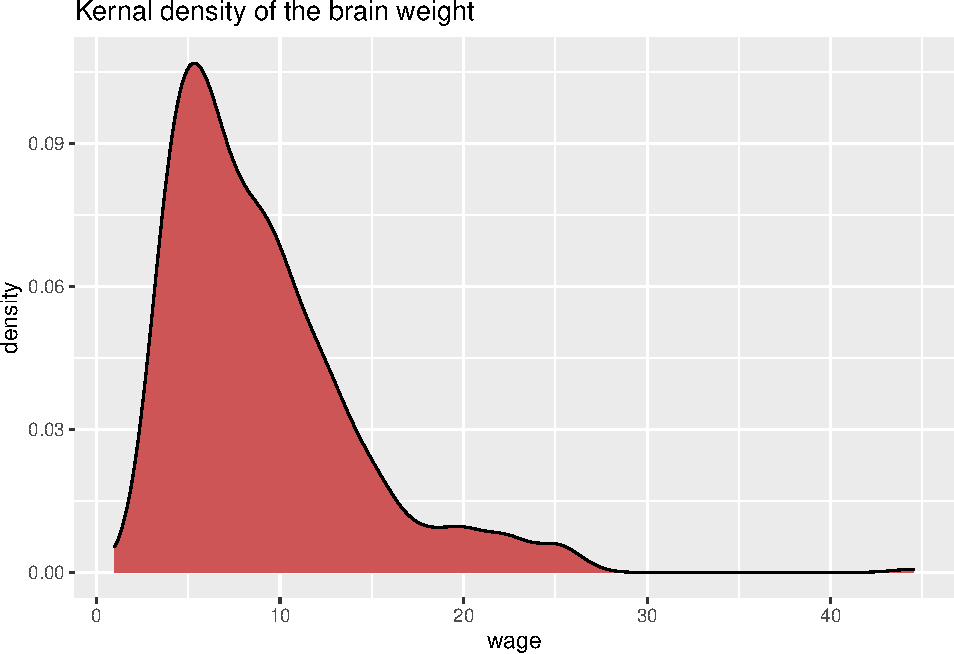
\includegraphics{17_1_21_files/figure-latex/unnamed-chunk-5-1.pdf}

\begin{Shaded}
\begin{Highlighting}[]
\CommentTok{\# Read car and truck values from tab{-}delimited autos.data}
\NormalTok{autos\_data }\OtherTok{\textless{}{-}} \FunctionTok{read.table}\NormalTok{(}\StringTok{"autos.dat"}\NormalTok{, }\AttributeTok{header=}\NormalTok{T, }\AttributeTok{sep=}\StringTok{"}\SpecialCharTok{\textbackslash{}t}\StringTok{"}\NormalTok{)}
\NormalTok{autos\_data}
\end{Highlighting}
\end{Shaded}

\begin{verbatim}
##   cars trucks suvs
## 1    1      2    4
## 2    3      5    4
## 3    6      4    6
## 4    4      5    6
## 5    9     12   16
\end{verbatim}

\begin{Shaded}
\begin{Highlighting}[]
\CommentTok{\# Compute the largest y value used in the data (or we could just use range again)}
\NormalTok{max\_y }\OtherTok{\textless{}{-}} \FunctionTok{max}\NormalTok{(autos\_data)}
\NormalTok{max\_y}
\end{Highlighting}
\end{Shaded}

\begin{verbatim}
## [1] 16
\end{verbatim}

\begin{Shaded}
\begin{Highlighting}[]
\CommentTok{\# Define colors to be used for cars, trucks, suvs}
\NormalTok{plot\_colors }\OtherTok{\textless{}{-}} \FunctionTok{c}\NormalTok{(}\StringTok{"blue"}\NormalTok{,}\StringTok{"red"}\NormalTok{,}\StringTok{"forestgreen"}\NormalTok{)}

\CommentTok{\# Start PNG device driver to save output to figure.png}
\FunctionTok{png}\NormalTok{(}\AttributeTok{filename=}\StringTok{"figure.png"}\NormalTok{, }\AttributeTok{height=}\DecValTok{295}\NormalTok{, }\AttributeTok{width=}\DecValTok{300}\NormalTok{, }\AttributeTok{bg=}\StringTok{"white"}\NormalTok{)}

\CommentTok{\# Graph autos using y axis that ranges from 0 to max\_y.}
\CommentTok{\# Turn off axes and annotations (axis labels) so we can specify them ourself}
\FunctionTok{plot}\NormalTok{(autos\_data}\SpecialCharTok{$}\NormalTok{cars, }\AttributeTok{type=}\StringTok{"o"}\NormalTok{, }\AttributeTok{col=}\NormalTok{plot\_colors[}\DecValTok{1}\NormalTok{], }\AttributeTok{ylim=}\FunctionTok{c}\NormalTok{(}\DecValTok{0}\NormalTok{,max\_y), }\AttributeTok{axes=}\ConstantTok{FALSE}\NormalTok{, }\AttributeTok{ann=}\ConstantTok{FALSE}\NormalTok{)}

\CommentTok{\# Make x axis using Mon{-}Fri labels}
\FunctionTok{axis}\NormalTok{(}\DecValTok{1}\NormalTok{, }\AttributeTok{at=}\DecValTok{1}\SpecialCharTok{:}\DecValTok{5}\NormalTok{, }\AttributeTok{lab=}\FunctionTok{c}\NormalTok{(}\StringTok{"Mon"}\NormalTok{, }\StringTok{"Tue"}\NormalTok{, }\StringTok{"Wed"}\NormalTok{, }\StringTok{"Thu"}\NormalTok{, }\StringTok{"Fri"}\NormalTok{))}

\CommentTok{\# Make y axis with horizontal labels that display ticks at every 4 marks. 4*0:max\_y is equivalent to c(0,4,8,12).}
\FunctionTok{axis}\NormalTok{(}\DecValTok{2}\NormalTok{, }\AttributeTok{las=}\DecValTok{1}\NormalTok{, }\AttributeTok{at=}\DecValTok{4}\SpecialCharTok{*}\DecValTok{0}\SpecialCharTok{:}\NormalTok{max\_y)}

\CommentTok{\# Create box around plot}
\FunctionTok{box}\NormalTok{()}

\CommentTok{\# Graph trucks with red dashed line and square points}
\FunctionTok{lines}\NormalTok{(autos\_data}\SpecialCharTok{$}\NormalTok{trucks, }\AttributeTok{type=}\StringTok{"o"}\NormalTok{, }\AttributeTok{pch=}\DecValTok{22}\NormalTok{, }\AttributeTok{lty=}\DecValTok{2}\NormalTok{, }\AttributeTok{col=}\NormalTok{plot\_colors[}\DecValTok{2}\NormalTok{])}

\CommentTok{\# Graph suvs with green dotted line and diamond points}
\FunctionTok{lines}\NormalTok{(autos\_data}\SpecialCharTok{$}\NormalTok{suvs, }\AttributeTok{type=}\StringTok{"o"}\NormalTok{, }\AttributeTok{pch=}\DecValTok{23}\NormalTok{, }\AttributeTok{lty=}\DecValTok{3}\NormalTok{, }\AttributeTok{col=}\NormalTok{plot\_colors[}\DecValTok{3}\NormalTok{])}

\CommentTok{\# Create a title with a red, bold/italic font}
\FunctionTok{title}\NormalTok{(}\AttributeTok{main=}\StringTok{"Autos"}\NormalTok{, }\AttributeTok{col.main=}\StringTok{"red"}\NormalTok{, }\AttributeTok{font.main=}\DecValTok{4}\NormalTok{)}

\CommentTok{\# Label the x and y axes with dark green text}
\FunctionTok{title}\NormalTok{(}\AttributeTok{xlab=} \StringTok{"Days"}\NormalTok{, }\AttributeTok{col.lab=}\FunctionTok{rgb}\NormalTok{(}\DecValTok{0}\NormalTok{,}\FloatTok{0.5}\NormalTok{,}\DecValTok{0}\NormalTok{))}
\FunctionTok{title}\NormalTok{(}\AttributeTok{ylab=} \StringTok{"Total"}\NormalTok{, }\AttributeTok{col.lab=}\FunctionTok{rgb}\NormalTok{(}\DecValTok{0}\NormalTok{,}\FloatTok{0.5}\NormalTok{,}\DecValTok{0}\NormalTok{))}

\CommentTok{\# Create a legend at (1, max\_y) that is slightly smaller (cex) and uses the same line colors and points used by the actual plots}
\FunctionTok{legend}\NormalTok{(}\DecValTok{1}\NormalTok{, max\_y, }\FunctionTok{names}\NormalTok{(autos\_data), }\AttributeTok{cex=}\FloatTok{0.8}\NormalTok{, }\AttributeTok{col=}\NormalTok{plot\_colors, }\AttributeTok{pch=}\DecValTok{21}\SpecialCharTok{:}\DecValTok{23}\NormalTok{, }\AttributeTok{lty=}\DecValTok{1}\SpecialCharTok{:}\DecValTok{3}\NormalTok{);}

\CommentTok{\# Turn off device driver (to flush output to png)}
\FunctionTok{dev.off}\NormalTok{()}
\end{Highlighting}
\end{Shaded}

\begin{verbatim}
## pdf 
##   2
\end{verbatim}

\begin{Shaded}
\begin{Highlighting}[]
\CommentTok{\# Define colors to be used for cars, trucks, suvs}
\NormalTok{plot\_colors }\OtherTok{\textless{}{-}} \FunctionTok{c}\NormalTok{(}\FunctionTok{rgb}\NormalTok{(}\AttributeTok{r=}\FloatTok{0.0}\NormalTok{,}\AttributeTok{g=}\FloatTok{0.0}\NormalTok{,}\AttributeTok{b=}\FloatTok{0.9}\NormalTok{), }\StringTok{"red"}\NormalTok{, }\StringTok{"forestgreen"}\NormalTok{)}

\CommentTok{\# Start PDF device driver to save output to figure.pdf}
\FunctionTok{pdf}\NormalTok{(}\AttributeTok{file=}\StringTok{"figure.pdf"}\NormalTok{, }\AttributeTok{height=}\FloatTok{3.5}\NormalTok{, }\AttributeTok{width=}\DecValTok{5}\NormalTok{)}

\CommentTok{\# Trim off excess margin space (bottom, left, top, right)}
\FunctionTok{par}\NormalTok{(}\AttributeTok{mar=}\FunctionTok{c}\NormalTok{(}\FloatTok{4.2}\NormalTok{, }\FloatTok{3.8}\NormalTok{, }\FloatTok{0.2}\NormalTok{, }\FloatTok{0.2}\NormalTok{))}

\CommentTok{\# Graph autos using a y axis that uses the full range of value in autos\_data. Label axes with smaller font and use larger line widths.}
\FunctionTok{plot}\NormalTok{(autos\_data}\SpecialCharTok{$}\NormalTok{cars, }\AttributeTok{type=}\StringTok{"l"}\NormalTok{, }\AttributeTok{col=}\NormalTok{plot\_colors[}\DecValTok{1}\NormalTok{],}
\AttributeTok{ylim =} \FunctionTok{range}\NormalTok{(autos\_data), }\AttributeTok{axes=}\NormalTok{F, }\AttributeTok{ann=}\NormalTok{T, }
\AttributeTok{xlab=}\StringTok{"Days"}\NormalTok{, }\AttributeTok{ylab=}\StringTok{"Total"}\NormalTok{, }\AttributeTok{cex.lab=}\FloatTok{0.8}\NormalTok{, }\AttributeTok{lwd=}\DecValTok{2}\NormalTok{)}

\CommentTok{\# Make x axis tick marks without labels}
\FunctionTok{axis}\NormalTok{(}\DecValTok{1}\NormalTok{, }\AttributeTok{lab=}\NormalTok{F)}

\CommentTok{\# Plot x axis labels at default tick marks with labels at 45 degree angle}
\FunctionTok{text}\NormalTok{(}\FunctionTok{axTicks}\NormalTok{(}\DecValTok{1}\NormalTok{), }\FunctionTok{par}\NormalTok{(}\StringTok{"usr"}\NormalTok{)[}\DecValTok{3}\NormalTok{] }\SpecialCharTok{{-}} \DecValTok{2}\NormalTok{, }\AttributeTok{srt=}\DecValTok{45}\NormalTok{, }\AttributeTok{adj=}\DecValTok{1}\NormalTok{, }\AttributeTok{labels=}\FunctionTok{c}\NormalTok{(}\StringTok{"Mon"}\NormalTok{, }\StringTok{"Tue"}\NormalTok{, }\StringTok{"Wed"}\NormalTok{, }\StringTok{"Thu"}\NormalTok{, }\StringTok{"Fri"}\NormalTok{), }\AttributeTok{xpd=}\NormalTok{T, }\AttributeTok{cex=}\FloatTok{0.8}\NormalTok{)}

\CommentTok{\# Plot y axis with smaller horizontal labels}
\FunctionTok{axis}\NormalTok{(}\DecValTok{2}\NormalTok{, }\AttributeTok{las=}\DecValTok{1}\NormalTok{, }\AttributeTok{cex.axis=}\FloatTok{0.8}\NormalTok{)}

\CommentTok{\# Create box around plot}
\FunctionTok{box}\NormalTok{()}

\CommentTok{\# Graph trucks with thicker red dashed line}
\FunctionTok{lines}\NormalTok{(autos\_data}\SpecialCharTok{$}\NormalTok{trucks, }\AttributeTok{type=}\StringTok{"l"}\NormalTok{, }\AttributeTok{lty=}\DecValTok{2}\NormalTok{, }\AttributeTok{lwd=}\DecValTok{2}\NormalTok{,}\AttributeTok{col=}\NormalTok{plot\_colors[}\DecValTok{2}\NormalTok{])}

\CommentTok{\# Graph suvs with thicker green dotted line}
\FunctionTok{lines}\NormalTok{(autos\_data}\SpecialCharTok{$}\NormalTok{suvs, }\AttributeTok{type=}\StringTok{"l"}\NormalTok{, }\AttributeTok{lty=}\DecValTok{3}\NormalTok{, }\AttributeTok{lwd=}\DecValTok{2}\NormalTok{, }\AttributeTok{col=}\NormalTok{plot\_colors[}\DecValTok{3}\NormalTok{])}

\CommentTok{\# Create a legend in the top{-}left corner that is slightly smaller and has no border}
\FunctionTok{legend}\NormalTok{(}\StringTok{"topleft"}\NormalTok{, }\FunctionTok{names}\NormalTok{(autos\_data), }\AttributeTok{cex=}\FloatTok{0.8}\NormalTok{, }\AttributeTok{col=}\NormalTok{plot\_colors, }\AttributeTok{lty=}\DecValTok{1}\SpecialCharTok{:}\DecValTok{3}\NormalTok{, }\AttributeTok{lwd=}\DecValTok{2}\NormalTok{, }\AttributeTok{bty=}\StringTok{"n"}\NormalTok{);}

\CommentTok{\# Turn off device driver (to flush output to PDF)}
\FunctionTok{dev.off}\NormalTok{()}
\end{Highlighting}
\end{Shaded}

\begin{verbatim}
## pdf 
##   2
\end{verbatim}

\begin{Shaded}
\begin{Highlighting}[]
\CommentTok{\# Restore default margins}
\FunctionTok{par}\NormalTok{(}\AttributeTok{mar=}\FunctionTok{c}\NormalTok{(}\DecValTok{5}\NormalTok{, }\DecValTok{4}\NormalTok{, }\DecValTok{4}\NormalTok{, }\DecValTok{2}\NormalTok{) }\SpecialCharTok{+} \FloatTok{0.1}\NormalTok{)}
\end{Highlighting}
\end{Shaded}

\hypertarget{bar-chart}{%
\subsection{Bar Chart}\label{bar-chart}}

\begin{Shaded}
\begin{Highlighting}[]
\CommentTok{\# Define the cars vector with 5 values}
\NormalTok{cars }\OtherTok{\textless{}{-}} \FunctionTok{c}\NormalTok{(}\DecValTok{1}\NormalTok{, }\DecValTok{3}\NormalTok{, }\DecValTok{6}\NormalTok{, }\DecValTok{4}\NormalTok{, }\DecValTok{9}\NormalTok{)}

\CommentTok{\# Graph cars}
\FunctionTok{barplot}\NormalTok{(cars)}
\end{Highlighting}
\end{Shaded}

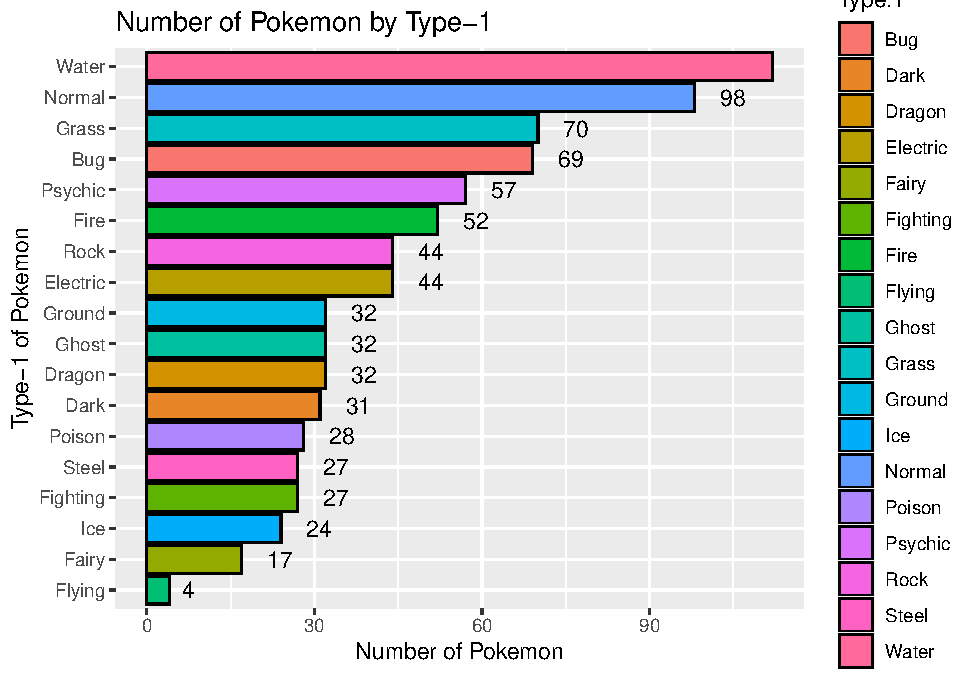
\includegraphics{17_1_21_files/figure-latex/unnamed-chunk-11-1.pdf}

\begin{Shaded}
\begin{Highlighting}[]
\CommentTok{\# Read values from tab{-}delimited autos.dat}
\NormalTok{autos\_data }\OtherTok{=} \FunctionTok{read.table}\NormalTok{(}\StringTok{"autos.dat"}\NormalTok{, }\AttributeTok{header=}\NormalTok{T, }\AttributeTok{sep=}\StringTok{"}\SpecialCharTok{\textbackslash{}t}\StringTok{"}\NormalTok{)}

\FunctionTok{barplot}\NormalTok{(autos\_data}\SpecialCharTok{$}\NormalTok{cars, }\AttributeTok{main=}\StringTok{"Cars"}\NormalTok{, }
\AttributeTok{xlab=}\StringTok{"Days"}\NormalTok{, }\AttributeTok{ylab=}\StringTok{"Total"}\NormalTok{, }\AttributeTok{names.arg=}\FunctionTok{c}\NormalTok{(}\StringTok{"Mon"}\NormalTok{,}\StringTok{"Tue"}\NormalTok{,}\StringTok{"Wed"}\NormalTok{,}\StringTok{"Thu"}\NormalTok{,}\StringTok{"Fri"}\NormalTok{),}
\AttributeTok{border=}\StringTok{"blue"}\NormalTok{, }\AttributeTok{density=}\FunctionTok{c}\NormalTok{(}\DecValTok{10}\NormalTok{,}\DecValTok{20}\NormalTok{,}\DecValTok{30}\NormalTok{,}\DecValTok{40}\NormalTok{,}\DecValTok{50}\NormalTok{))}
\end{Highlighting}
\end{Shaded}

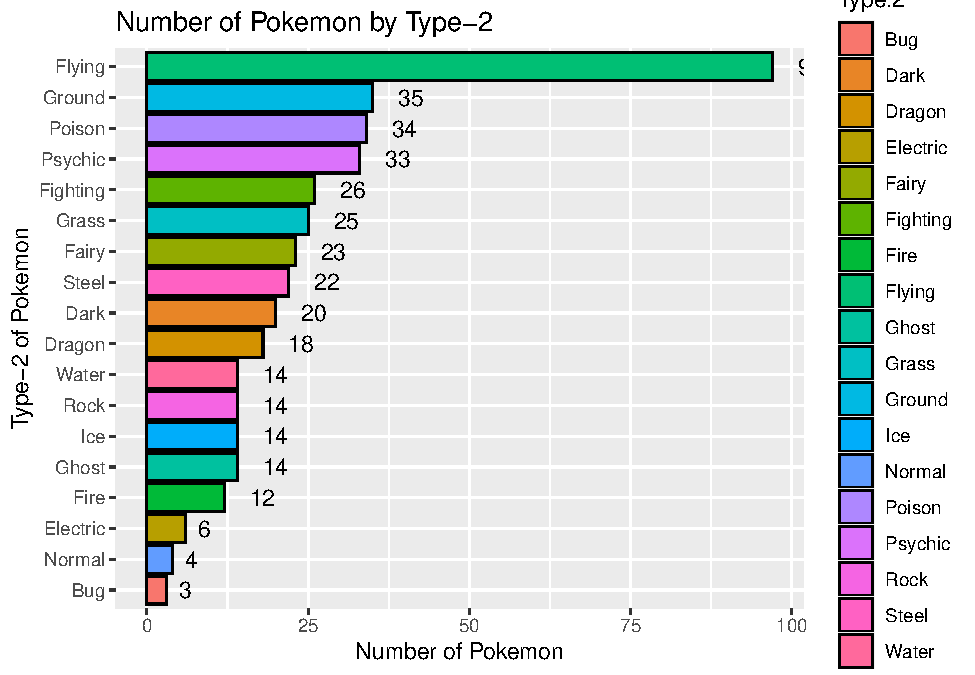
\includegraphics{17_1_21_files/figure-latex/unnamed-chunk-12-1.pdf}

\begin{Shaded}
\begin{Highlighting}[]
\FunctionTok{matrix}\NormalTok{(autos\_data)}
\end{Highlighting}
\end{Shaded}

\begin{verbatim}
##      [,1]     
## [1,] integer,5
## [2,] integer,5
## [3,] integer,5
\end{verbatim}

\begin{Shaded}
\begin{Highlighting}[]
\CommentTok{\# Graph autos with adjacent bars using rainbow colors}
\FunctionTok{barplot}\NormalTok{(}\FunctionTok{as.matrix}\NormalTok{(autos\_data), }\AttributeTok{main=}\StringTok{"Autos"}\NormalTok{, }\AttributeTok{ylab=} \StringTok{"Total"}\NormalTok{,}\AttributeTok{beside=}\ConstantTok{TRUE}\NormalTok{, }\AttributeTok{col=}\FunctionTok{rainbow}\NormalTok{(}\DecValTok{5}\NormalTok{))}

\CommentTok{\# Place the legend at the top{-}left corner with no frame using rainbow colors}
\FunctionTok{legend}\NormalTok{(}\StringTok{"topleft"}\NormalTok{, }\FunctionTok{c}\NormalTok{(}\StringTok{"Mon"}\NormalTok{,}\StringTok{"Tue"}\NormalTok{,}\StringTok{"Wed"}\NormalTok{,}\StringTok{"Thu"}\NormalTok{,}\StringTok{"Fri"}\NormalTok{), }\AttributeTok{cex=}\FloatTok{0.6}\NormalTok{, }\AttributeTok{bty=}\StringTok{"n"}\NormalTok{, }\AttributeTok{fill=}\FunctionTok{rainbow}\NormalTok{(}\DecValTok{5}\NormalTok{));}
\end{Highlighting}
\end{Shaded}

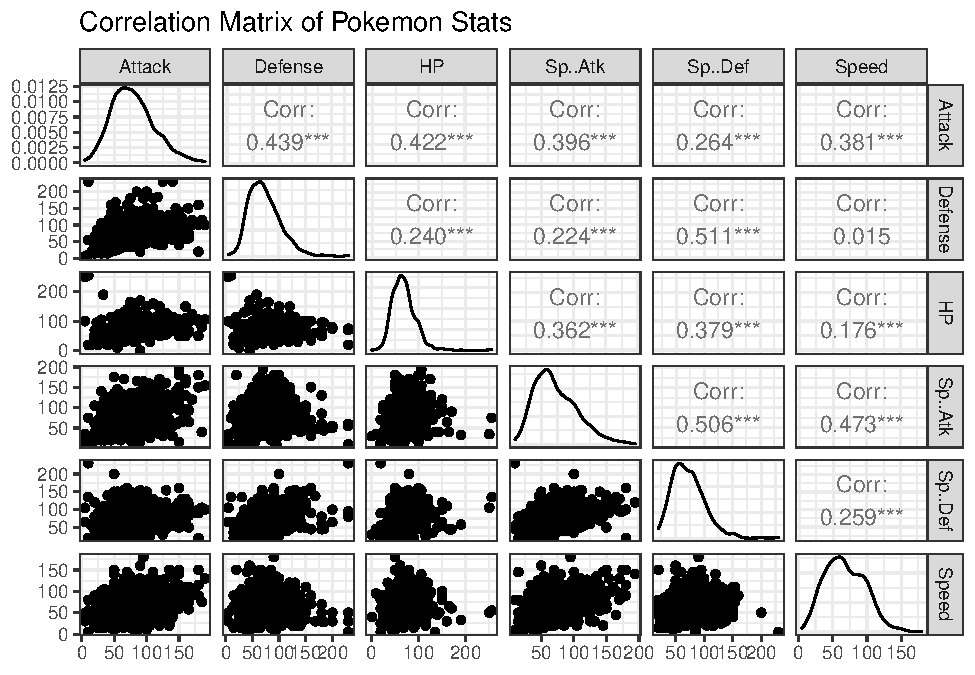
\includegraphics{17_1_21_files/figure-latex/unnamed-chunk-14-1.pdf}

\begin{Shaded}
\begin{Highlighting}[]
\CommentTok{\# Expand right side of clipping rect to make room for the legend}
\FunctionTok{par}\NormalTok{(}\AttributeTok{xpd=}\NormalTok{T, }\AttributeTok{mar=}\FunctionTok{par}\NormalTok{()}\SpecialCharTok{$}\NormalTok{mar}\SpecialCharTok{+}\FunctionTok{c}\NormalTok{(}\DecValTok{0}\NormalTok{,}\DecValTok{0}\NormalTok{,}\DecValTok{0}\NormalTok{,}\DecValTok{4}\NormalTok{))}

\CommentTok{\# Graph autos (transposing the matrix) using heat colors,}
\CommentTok{\# put 10\% of the space between each bar, and make labels smaller with horizontal y{-}axis labels}
\FunctionTok{barplot}\NormalTok{(}\FunctionTok{t}\NormalTok{(autos\_data), }\AttributeTok{main=}\StringTok{"Autos"}\NormalTok{, }\AttributeTok{ylab=}\StringTok{"Total"}\NormalTok{,}\AttributeTok{col=}\FunctionTok{heat.colors}\NormalTok{(}\DecValTok{3}\NormalTok{), }\AttributeTok{space=}\FloatTok{0.1}\NormalTok{, }\AttributeTok{cex.axis=}\FloatTok{0.8}\NormalTok{, }\AttributeTok{las=}\DecValTok{1}\NormalTok{,}
\AttributeTok{names.arg =} \FunctionTok{c}\NormalTok{(}\StringTok{"Mon"}\NormalTok{,}\StringTok{"Tue"}\NormalTok{,}\StringTok{"Wed"}\NormalTok{,}\StringTok{"Thu"}\NormalTok{,}\StringTok{"Fri"}\NormalTok{),}\AttributeTok{cex=}\FloatTok{0.8}\NormalTok{)}

\CommentTok{\# Place the legend at (6,30) using heat colors}
\FunctionTok{legend}\NormalTok{(}\DecValTok{6}\NormalTok{, }\DecValTok{30}\NormalTok{, }\FunctionTok{names}\NormalTok{(autos\_data), }\AttributeTok{cex=}\FloatTok{0.8}\NormalTok{, }\AttributeTok{fill=}\FunctionTok{heat.colors}\NormalTok{(}\DecValTok{3}\NormalTok{));}
\end{Highlighting}
\end{Shaded}

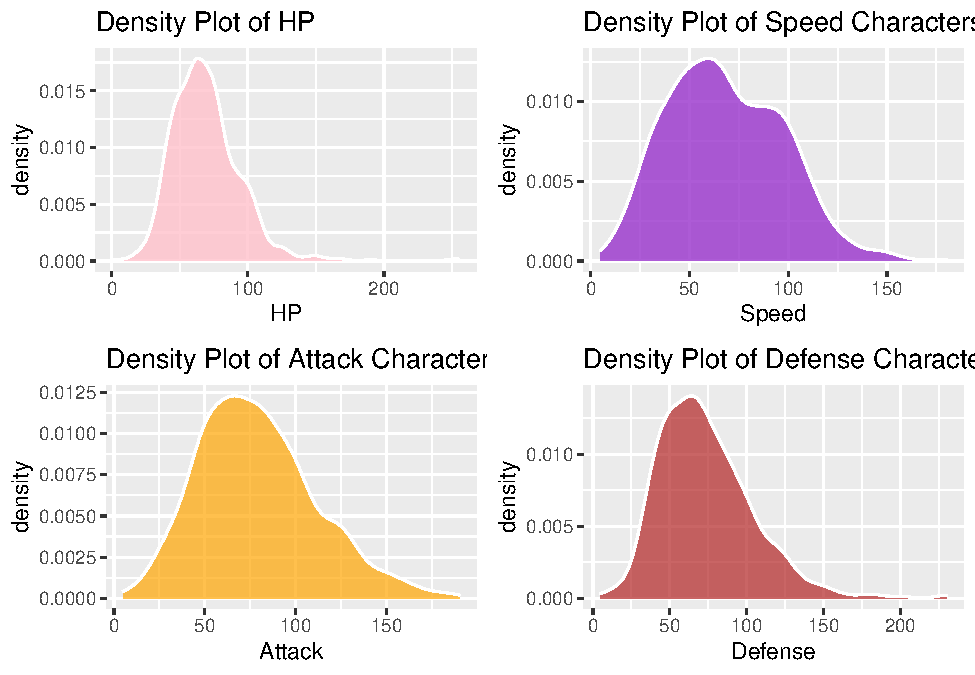
\includegraphics{17_1_21_files/figure-latex/unnamed-chunk-15-1.pdf}

\begin{Shaded}
\begin{Highlighting}[]
\CommentTok{\# Restore default clipping rect}
\FunctionTok{par}\NormalTok{(}\AttributeTok{mar=}\FunctionTok{c}\NormalTok{(}\DecValTok{5}\NormalTok{, }\DecValTok{4}\NormalTok{, }\DecValTok{4}\NormalTok{, }\DecValTok{2}\NormalTok{) }\SpecialCharTok{+} \FloatTok{0.1}\NormalTok{)}
\end{Highlighting}
\end{Shaded}

\hypertarget{histograms}{%
\subsection{Histograms}\label{histograms}}

\begin{Shaded}
\begin{Highlighting}[]
\CommentTok{\# Define the suvs vector with 5 values}
\NormalTok{suvs }\OtherTok{\textless{}{-}} \FunctionTok{c}\NormalTok{(}\DecValTok{4}\NormalTok{,}\DecValTok{4}\NormalTok{,}\DecValTok{6}\NormalTok{,}\DecValTok{6}\NormalTok{,}\DecValTok{16}\NormalTok{)}

\CommentTok{\# Create a histogram for suvs}
\FunctionTok{hist}\NormalTok{(suvs)}
\end{Highlighting}
\end{Shaded}

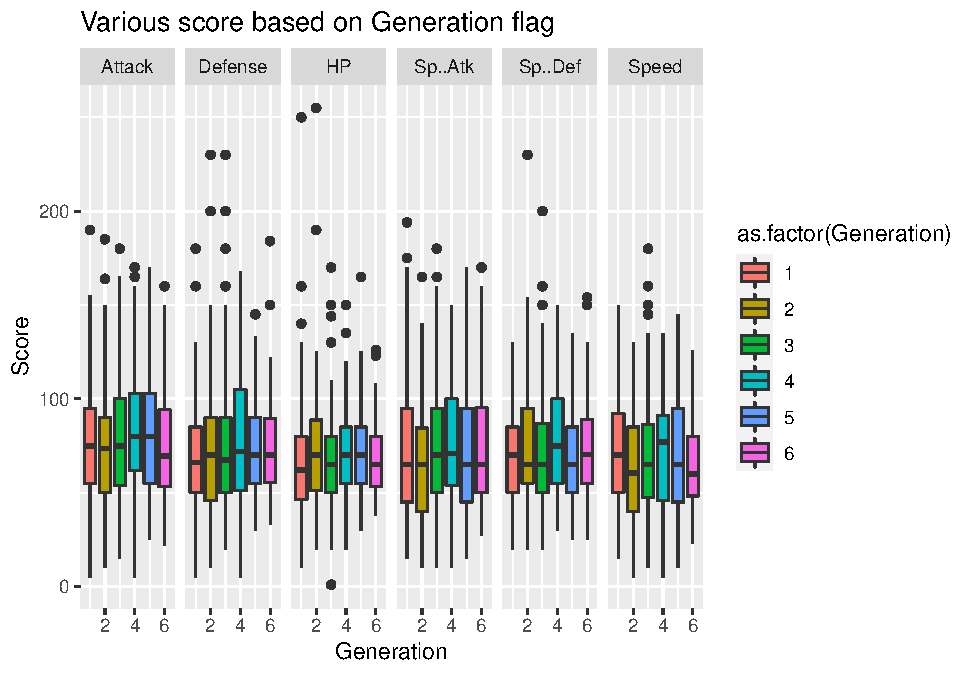
\includegraphics{17_1_21_files/figure-latex/unnamed-chunk-16-1.pdf}

\begin{Shaded}
\begin{Highlighting}[]
\CommentTok{\# Concatenate the three vectors}
\NormalTok{autos }\OtherTok{\textless{}{-}} \FunctionTok{c}\NormalTok{(autos\_data}\SpecialCharTok{$}\NormalTok{cars, autos\_data}\SpecialCharTok{$}\NormalTok{trucks, autos\_data}\SpecialCharTok{$}\NormalTok{suvs)}

\CommentTok{\# Create a histogram for autos in light blue with the y axis ranging from 0{-}10}
\FunctionTok{hist}\NormalTok{(autos, }\AttributeTok{col=}\StringTok{"lightblue"}\NormalTok{, }\AttributeTok{ylim=}\FunctionTok{c}\NormalTok{(}\DecValTok{0}\NormalTok{,}\DecValTok{10}\NormalTok{))}
\end{Highlighting}
\end{Shaded}

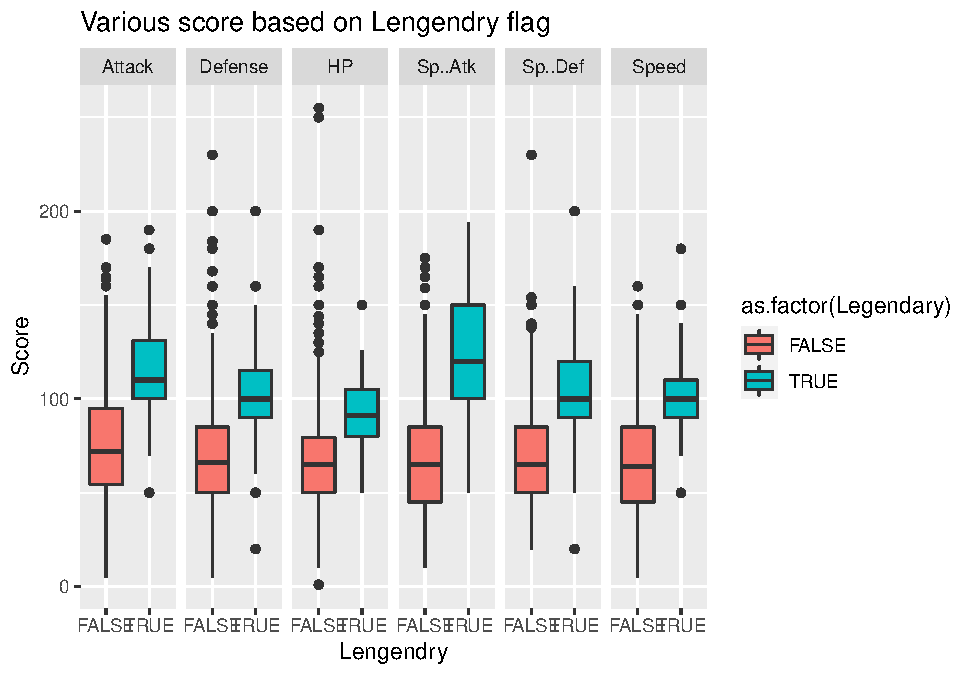
\includegraphics{17_1_21_files/figure-latex/unnamed-chunk-17-1.pdf}

\begin{Shaded}
\begin{Highlighting}[]
\CommentTok{\# Concatenate the three vectors}
\NormalTok{autos }\OtherTok{\textless{}{-}} \FunctionTok{c}\NormalTok{(autos\_data}\SpecialCharTok{$}\NormalTok{cars, autos\_data}\SpecialCharTok{$}\NormalTok{trucks,autos\_data}\SpecialCharTok{$}\NormalTok{suvs)}

\CommentTok{\# Compute the largest y value used in the autos}
\NormalTok{max\_num }\OtherTok{\textless{}{-}} \FunctionTok{max}\NormalTok{(autos)}
\FunctionTok{hist}\NormalTok{(autos, }\AttributeTok{col=}\FunctionTok{heat.colors}\NormalTok{(max\_num), }\AttributeTok{breaks=}\NormalTok{max\_num,}
\AttributeTok{xlim=}\FunctionTok{c}\NormalTok{(}\DecValTok{0}\NormalTok{,max\_num), }\AttributeTok{right=}\NormalTok{F, }\AttributeTok{main=}\StringTok{"Autos Histogram"}\NormalTok{, }\AttributeTok{las=}\DecValTok{1}\NormalTok{)}
\end{Highlighting}
\end{Shaded}

\includegraphics{17_1_21_files/figure-latex/unnamed-chunk-18-1.pdf}

\begin{Shaded}
\begin{Highlighting}[]
\CommentTok{\# Concatenate the three vectors}
\NormalTok{autos }\OtherTok{\textless{}{-}} \FunctionTok{c}\NormalTok{(autos\_data}\SpecialCharTok{$}\NormalTok{cars, autos\_data}\SpecialCharTok{$}\NormalTok{trucks,}
\NormalTok{autos\_data}\SpecialCharTok{$}\NormalTok{suvs)}

\CommentTok{\# Compute the largest y value used in the autos}
\NormalTok{max\_num }\OtherTok{\textless{}{-}} \FunctionTok{max}\NormalTok{(autos)}

\CommentTok{\# Create uneven breaks}
\NormalTok{brk }\OtherTok{\textless{}{-}} \FunctionTok{c}\NormalTok{(}\DecValTok{0}\NormalTok{,}\DecValTok{3}\NormalTok{,}\DecValTok{4}\NormalTok{,}\DecValTok{5}\NormalTok{,}\DecValTok{6}\NormalTok{,}\DecValTok{10}\NormalTok{,}\DecValTok{16}\NormalTok{)}

\FunctionTok{hist}\NormalTok{(autos, }\AttributeTok{col=}\FunctionTok{heat.colors}\NormalTok{(}\FunctionTok{length}\NormalTok{(brk)), }\AttributeTok{breaks=}\NormalTok{brk,}\AttributeTok{xlim=}\FunctionTok{c}\NormalTok{(}\DecValTok{0}\NormalTok{,max\_num), }\AttributeTok{right=}\NormalTok{F, }\AttributeTok{main=}\StringTok{"Probability Density"}\NormalTok{,}\AttributeTok{las=}\DecValTok{1}\NormalTok{, }\AttributeTok{cex.axis=}\FloatTok{0.8}\NormalTok{,}\AttributeTok{freq=}\NormalTok{F)}
\end{Highlighting}
\end{Shaded}

\includegraphics{17_1_21_files/figure-latex/unnamed-chunk-19-1.pdf}

\begin{Shaded}
\begin{Highlighting}[]
\CommentTok{\# Get a random log{-}normal distribution}
\NormalTok{r }\OtherTok{\textless{}{-}} \FunctionTok{rlnorm}\NormalTok{(}\DecValTok{1000}\NormalTok{)}
\FunctionTok{hist}\NormalTok{(r)}
\end{Highlighting}
\end{Shaded}

\includegraphics{17_1_21_files/figure-latex/unnamed-chunk-20-1.pdf}

\begin{Shaded}
\begin{Highlighting}[]
\CommentTok{\# Get a random log{-}normal distribution}
\NormalTok{r }\OtherTok{\textless{}{-}} \FunctionTok{rlnorm}\NormalTok{(}\DecValTok{1000}\NormalTok{)}

\CommentTok{\# Get the distribution without plotting it using tighter breaks}
\NormalTok{h }\OtherTok{\textless{}{-}} \FunctionTok{hist}\NormalTok{(r, }\AttributeTok{plot=}\NormalTok{F, }\AttributeTok{breaks=}\FunctionTok{c}\NormalTok{(}\FunctionTok{seq}\NormalTok{(}\DecValTok{0}\NormalTok{,}\FunctionTok{max}\NormalTok{(r)}\SpecialCharTok{+}\DecValTok{1}\NormalTok{, .}\DecValTok{1}\NormalTok{)))}

\NormalTok{h}
\end{Highlighting}
\end{Shaded}

\begin{verbatim}
## $breaks
##   [1]  0.0  0.1  0.2  0.3  0.4  0.5  0.6  0.7  0.8  0.9  1.0  1.1  1.2  1.3  1.4
##  [16]  1.5  1.6  1.7  1.8  1.9  2.0  2.1  2.2  2.3  2.4  2.5  2.6  2.7  2.8  2.9
##  [31]  3.0  3.1  3.2  3.3  3.4  3.5  3.6  3.7  3.8  3.9  4.0  4.1  4.2  4.3  4.4
##  [46]  4.5  4.6  4.7  4.8  4.9  5.0  5.1  5.2  5.3  5.4  5.5  5.6  5.7  5.8  5.9
##  [61]  6.0  6.1  6.2  6.3  6.4  6.5  6.6  6.7  6.8  6.9  7.0  7.1  7.2  7.3  7.4
##  [76]  7.5  7.6  7.7  7.8  7.9  8.0  8.1  8.2  8.3  8.4  8.5  8.6  8.7  8.8  8.9
##  [91]  9.0  9.1  9.2  9.3  9.4  9.5  9.6  9.7  9.8  9.9 10.0 10.1 10.2 10.3 10.4
## [106] 10.5 10.6 10.7 10.8 10.9 11.0 11.1 11.2 11.3 11.4 11.5 11.6 11.7 11.8 11.9
## [121] 12.0 12.1 12.2 12.3 12.4 12.5 12.6 12.7 12.8 12.9 13.0 13.1 13.2 13.3 13.4
## [136] 13.5 13.6 13.7 13.8 13.9 14.0 14.1 14.2 14.3 14.4 14.5 14.6 14.7 14.8 14.9
## [151] 15.0 15.1 15.2 15.3 15.4 15.5 15.6 15.7 15.8 15.9 16.0 16.1 16.2 16.3 16.4
## [166] 16.5 16.6 16.7 16.8 16.9 17.0 17.1 17.2 17.3 17.4 17.5 17.6 17.7 17.8 17.9
## [181] 18.0 18.1 18.2 18.3 18.4 18.5 18.6 18.7 18.8 18.9 19.0 19.1 19.2 19.3 19.4
## [196] 19.5 19.6 19.7 19.8 19.9 20.0 20.1 20.2 20.3 20.4 20.5 20.6 20.7 20.8 20.9
## [211] 21.0 21.1 21.2 21.3 21.4 21.5 21.6 21.7 21.8 21.9 22.0 22.1 22.2 22.3 22.4
## [226] 22.5
## 
## $counts
##   [1] 12 37 50 81 69 58 57 57 52 37 32 39 22 33 21 31 14 21 15 14 17 14 12 11 13
##  [26]  6  7  6  7 12  7  5  2  7  2  4  3  7  4  8  3  6  6  7  1  0  4  5  3  1
##  [51]  2  5  1  2  2  1  2  1  0  0  0  1  3  1  2  0  1  1  0  1  1  2  0  2  1
##  [76]  0  1  1  1  1  0  1  1  0  1  1  0  0  1  0  0  3  0  0  0  0  0  0  1  0
## [101]  0  0  2  2  0  0  0  0  0  1  0  0  0  0  0  1  0  0  0  0  0  0  0  0  0
## [126]  1  0  0  0  0  0  0  0  0  1  0  1  0  0  0  0  0  0  0  0  0  0  0  0  0
## [151]  0  1  0  0  0  0  0  0  0  0  0  0  0  0  0  0  0  0  0  0  0  0  0  0  0
## [176]  0  0  0  0  0  0  0  0  0  0  0  0  0  0  0  0  0  0  0  0  0  0  0  0  0
## [201]  1  0  0  0  0  1  0  0  0  0  0  0  0  0  0  1  0  0  0  0  0  0  0  0  0
## 
## $density
##   [1] 0.12 0.37 0.50 0.81 0.69 0.58 0.57 0.57 0.52 0.37 0.32 0.39 0.22 0.33 0.21
##  [16] 0.31 0.14 0.21 0.15 0.14 0.17 0.14 0.12 0.11 0.13 0.06 0.07 0.06 0.07 0.12
##  [31] 0.07 0.05 0.02 0.07 0.02 0.04 0.03 0.07 0.04 0.08 0.03 0.06 0.06 0.07 0.01
##  [46] 0.00 0.04 0.05 0.03 0.01 0.02 0.05 0.01 0.02 0.02 0.01 0.02 0.01 0.00 0.00
##  [61] 0.00 0.01 0.03 0.01 0.02 0.00 0.01 0.01 0.00 0.01 0.01 0.02 0.00 0.02 0.01
##  [76] 0.00 0.01 0.01 0.01 0.01 0.00 0.01 0.01 0.00 0.01 0.01 0.00 0.00 0.01 0.00
##  [91] 0.00 0.03 0.00 0.00 0.00 0.00 0.00 0.00 0.01 0.00 0.00 0.00 0.02 0.02 0.00
## [106] 0.00 0.00 0.00 0.00 0.01 0.00 0.00 0.00 0.00 0.00 0.01 0.00 0.00 0.00 0.00
## [121] 0.00 0.00 0.00 0.00 0.00 0.01 0.00 0.00 0.00 0.00 0.00 0.00 0.00 0.00 0.01
## [136] 0.00 0.01 0.00 0.00 0.00 0.00 0.00 0.00 0.00 0.00 0.00 0.00 0.00 0.00 0.00
## [151] 0.00 0.01 0.00 0.00 0.00 0.00 0.00 0.00 0.00 0.00 0.00 0.00 0.00 0.00 0.00
## [166] 0.00 0.00 0.00 0.00 0.00 0.00 0.00 0.00 0.00 0.00 0.00 0.00 0.00 0.00 0.00
## [181] 0.00 0.00 0.00 0.00 0.00 0.00 0.00 0.00 0.00 0.00 0.00 0.00 0.00 0.00 0.00
## [196] 0.00 0.00 0.00 0.00 0.00 0.01 0.00 0.00 0.00 0.00 0.01 0.00 0.00 0.00 0.00
## [211] 0.00 0.00 0.00 0.00 0.00 0.01 0.00 0.00 0.00 0.00 0.00 0.00 0.00 0.00 0.00
## 
## $mids
##   [1]  0.05  0.15  0.25  0.35  0.45  0.55  0.65  0.75  0.85  0.95  1.05  1.15
##  [13]  1.25  1.35  1.45  1.55  1.65  1.75  1.85  1.95  2.05  2.15  2.25  2.35
##  [25]  2.45  2.55  2.65  2.75  2.85  2.95  3.05  3.15  3.25  3.35  3.45  3.55
##  [37]  3.65  3.75  3.85  3.95  4.05  4.15  4.25  4.35  4.45  4.55  4.65  4.75
##  [49]  4.85  4.95  5.05  5.15  5.25  5.35  5.45  5.55  5.65  5.75  5.85  5.95
##  [61]  6.05  6.15  6.25  6.35  6.45  6.55  6.65  6.75  6.85  6.95  7.05  7.15
##  [73]  7.25  7.35  7.45  7.55  7.65  7.75  7.85  7.95  8.05  8.15  8.25  8.35
##  [85]  8.45  8.55  8.65  8.75  8.85  8.95  9.05  9.15  9.25  9.35  9.45  9.55
##  [97]  9.65  9.75  9.85  9.95 10.05 10.15 10.25 10.35 10.45 10.55 10.65 10.75
## [109] 10.85 10.95 11.05 11.15 11.25 11.35 11.45 11.55 11.65 11.75 11.85 11.95
## [121] 12.05 12.15 12.25 12.35 12.45 12.55 12.65 12.75 12.85 12.95 13.05 13.15
## [133] 13.25 13.35 13.45 13.55 13.65 13.75 13.85 13.95 14.05 14.15 14.25 14.35
## [145] 14.45 14.55 14.65 14.75 14.85 14.95 15.05 15.15 15.25 15.35 15.45 15.55
## [157] 15.65 15.75 15.85 15.95 16.05 16.15 16.25 16.35 16.45 16.55 16.65 16.75
## [169] 16.85 16.95 17.05 17.15 17.25 17.35 17.45 17.55 17.65 17.75 17.85 17.95
## [181] 18.05 18.15 18.25 18.35 18.45 18.55 18.65 18.75 18.85 18.95 19.05 19.15
## [193] 19.25 19.35 19.45 19.55 19.65 19.75 19.85 19.95 20.05 20.15 20.25 20.35
## [205] 20.45 20.55 20.65 20.75 20.85 20.95 21.05 21.15 21.25 21.35 21.45 21.55
## [217] 21.65 21.75 21.85 21.95 22.05 22.15 22.25 22.35 22.45
## 
## $xname
## [1] "r"
## 
## $equidist
## [1] TRUE
## 
## attr(,"class")
## [1] "histogram"
\end{verbatim}

\begin{Shaded}
\begin{Highlighting}[]
\CommentTok{\# Plot the distribution using log scale on both axes, and use blue points}
\FunctionTok{plot}\NormalTok{(h}\SpecialCharTok{$}\NormalTok{counts, }\AttributeTok{log=}\StringTok{"xy"}\NormalTok{, }\AttributeTok{pch=}\DecValTok{20}\NormalTok{, }\AttributeTok{col=}\StringTok{"blue"}\NormalTok{, }\AttributeTok{main=}\StringTok{"Log{-}normal distribution"}\NormalTok{, }\AttributeTok{xlab=}\StringTok{"Value"}\NormalTok{, }\AttributeTok{ylab=}\StringTok{"Frequency"}\NormalTok{)}
\end{Highlighting}
\end{Shaded}

\begin{verbatim}
## Warning in xy.coords(x, y, xlabel, ylabel, log): 135 y values <= 0 omitted from
## logarithmic plot
\end{verbatim}

\includegraphics{17_1_21_files/figure-latex/unnamed-chunk-22-1.pdf}

\hypertarget{pie-chats}{%
\subsection{Pie Chats}\label{pie-chats}}

\begin{Shaded}
\begin{Highlighting}[]
\CommentTok{\# Define cars vector with 5 values}
\NormalTok{cars }\OtherTok{\textless{}{-}} \FunctionTok{c}\NormalTok{(}\DecValTok{1}\NormalTok{, }\DecValTok{3}\NormalTok{, }\DecValTok{6}\NormalTok{, }\DecValTok{4}\NormalTok{, }\DecValTok{9}\NormalTok{)}

\CommentTok{\# Create a pie chart for cars}
\FunctionTok{pie}\NormalTok{(cars)}
\end{Highlighting}
\end{Shaded}

\includegraphics{17_1_21_files/figure-latex/unnamed-chunk-23-1.pdf}

\begin{Shaded}
\begin{Highlighting}[]
\FunctionTok{pie}\NormalTok{(cars, }\AttributeTok{main=}\StringTok{"Cars"}\NormalTok{, }\AttributeTok{col=}\FunctionTok{rainbow}\NormalTok{(}\FunctionTok{length}\NormalTok{(cars)),}\AttributeTok{labels=}\FunctionTok{c}\NormalTok{(}\StringTok{"Mon"}\NormalTok{,}\StringTok{"Tue"}\NormalTok{,}\StringTok{"Wed"}\NormalTok{,}\StringTok{"Thu"}\NormalTok{,}\StringTok{"Fri"}\NormalTok{))}
\end{Highlighting}
\end{Shaded}

\includegraphics{17_1_21_files/figure-latex/unnamed-chunk-24-1.pdf}

\begin{Shaded}
\begin{Highlighting}[]
\CommentTok{\# Define some colors ideal for black \& white print}
\NormalTok{colors }\OtherTok{\textless{}{-}} \FunctionTok{c}\NormalTok{(}\StringTok{"white"}\NormalTok{,}\StringTok{"grey70"}\NormalTok{,}\StringTok{"grey90"}\NormalTok{,}\StringTok{"grey50"}\NormalTok{,}\StringTok{"black"}\NormalTok{)}

\CommentTok{\# Calculate the percentage for each day, rounded to one decimal place}
\NormalTok{car\_labels }\OtherTok{\textless{}{-}} \FunctionTok{round}\NormalTok{(cars}\SpecialCharTok{/}\FunctionTok{sum}\NormalTok{(cars) }\SpecialCharTok{*} \DecValTok{100}\NormalTok{, }\DecValTok{1}\NormalTok{)}

\CommentTok{\# Concatenate a \textquotesingle{}\%\textquotesingle{} char after each value}
\NormalTok{car\_labels }\OtherTok{\textless{}{-}} \FunctionTok{paste}\NormalTok{(car\_labels, }\StringTok{"\%"}\NormalTok{, }\AttributeTok{sep=}\StringTok{""}\NormalTok{)}

\CommentTok{\# Create a pie chart with defined heading and custom colors and labels}
\FunctionTok{pie}\NormalTok{(cars, }\AttributeTok{main=}\StringTok{"Cars"}\NormalTok{, }\AttributeTok{col=}\NormalTok{colors, }\AttributeTok{labels=}\NormalTok{car\_labels, }\AttributeTok{cex=}\FloatTok{0.8}\NormalTok{)}

\CommentTok{\# Create a legend at the right}
\FunctionTok{legend}\NormalTok{(}\FloatTok{1.5}\NormalTok{, }\FloatTok{0.5}\NormalTok{, }\FunctionTok{c}\NormalTok{(}\StringTok{"Mon"}\NormalTok{,}\StringTok{"Tue"}\NormalTok{,}\StringTok{"Wed"}\NormalTok{,}\StringTok{"Thu"}\NormalTok{,}\StringTok{"Fri"}\NormalTok{), }\AttributeTok{cex=}\FloatTok{0.8}\NormalTok{, }\AttributeTok{fill=}\NormalTok{colors)}
\end{Highlighting}
\end{Shaded}

\includegraphics{17_1_21_files/figure-latex/unnamed-chunk-25-1.pdf} \#\#
DotCharts

\begin{Shaded}
\begin{Highlighting}[]
\CommentTok{\# Create a dotchart for autos}
\FunctionTok{dotchart}\NormalTok{(}\FunctionTok{t}\NormalTok{(autos\_data))}
\end{Highlighting}
\end{Shaded}

\includegraphics{17_1_21_files/figure-latex/unnamed-chunk-26-1.pdf}

\begin{Shaded}
\begin{Highlighting}[]
\CommentTok{\# Create a colored dot{-}chart for autos with smaller labels}
\FunctionTok{dotchart}\NormalTok{(}\FunctionTok{t}\NormalTok{(autos\_data), }\AttributeTok{color=}\FunctionTok{c}\NormalTok{(}\StringTok{"red"}\NormalTok{,}\StringTok{"blue"}\NormalTok{,}\StringTok{"darkgreen"}\NormalTok{),}\AttributeTok{main=}\StringTok{"Dotchart for Autos"}\NormalTok{, }\AttributeTok{cex=}\FloatTok{0.8}\NormalTok{)}
\end{Highlighting}
\end{Shaded}

\includegraphics{17_1_21_files/figure-latex/unnamed-chunk-27-1.pdf} \#\#
MISC

\begin{Shaded}
\begin{Highlighting}[]
\CommentTok{\# Make an empty chart}
\FunctionTok{plot}\NormalTok{(}\DecValTok{1}\NormalTok{, }\DecValTok{1}\NormalTok{, }\AttributeTok{xlim=}\FunctionTok{c}\NormalTok{(}\DecValTok{1}\NormalTok{,}\FloatTok{5.5}\NormalTok{), }\AttributeTok{ylim=}\FunctionTok{c}\NormalTok{(}\DecValTok{0}\NormalTok{,}\DecValTok{7}\NormalTok{), }\AttributeTok{type=}\StringTok{"n"}\NormalTok{, }\AttributeTok{ann=}\ConstantTok{FALSE}\NormalTok{)}

\CommentTok{\# Plot digits 0{-}4 with increasing size and color}
\FunctionTok{text}\NormalTok{(}\DecValTok{1}\SpecialCharTok{:}\DecValTok{5}\NormalTok{, }\FunctionTok{rep}\NormalTok{(}\DecValTok{6}\NormalTok{,}\DecValTok{5}\NormalTok{), }\AttributeTok{labels=}\FunctionTok{c}\NormalTok{(}\DecValTok{0}\SpecialCharTok{:}\DecValTok{4}\NormalTok{), }\AttributeTok{cex=}\DecValTok{1}\SpecialCharTok{:}\DecValTok{5}\NormalTok{, }\AttributeTok{col=}\DecValTok{1}\SpecialCharTok{:}\DecValTok{5}\NormalTok{)}

\CommentTok{\# Plot symbols 0{-}4 with increasing size and color}
\FunctionTok{points}\NormalTok{(}\DecValTok{1}\SpecialCharTok{:}\DecValTok{5}\NormalTok{, }\FunctionTok{rep}\NormalTok{(}\DecValTok{5}\NormalTok{,}\DecValTok{5}\NormalTok{), }\AttributeTok{cex=}\DecValTok{1}\SpecialCharTok{:}\DecValTok{5}\NormalTok{, }\AttributeTok{col=}\DecValTok{1}\SpecialCharTok{:}\DecValTok{5}\NormalTok{, }\AttributeTok{pch=}\DecValTok{0}\SpecialCharTok{:}\DecValTok{4}\NormalTok{)}
\FunctionTok{text}\NormalTok{((}\DecValTok{1}\SpecialCharTok{:}\DecValTok{5}\NormalTok{)}\SpecialCharTok{+}\FloatTok{0.4}\NormalTok{, }\FunctionTok{rep}\NormalTok{(}\DecValTok{5}\NormalTok{,}\DecValTok{5}\NormalTok{), }\AttributeTok{cex=}\FloatTok{0.6}\NormalTok{, (}\DecValTok{0}\SpecialCharTok{:}\DecValTok{4}\NormalTok{))}

\CommentTok{\# Plot symbols 5{-}9 with labels}
\FunctionTok{points}\NormalTok{(}\DecValTok{1}\SpecialCharTok{:}\DecValTok{5}\NormalTok{, }\FunctionTok{rep}\NormalTok{(}\DecValTok{4}\NormalTok{,}\DecValTok{5}\NormalTok{), }\AttributeTok{cex=}\DecValTok{2}\NormalTok{, }\AttributeTok{pch=}\NormalTok{(}\DecValTok{5}\SpecialCharTok{:}\DecValTok{9}\NormalTok{))}
\FunctionTok{text}\NormalTok{((}\DecValTok{1}\SpecialCharTok{:}\DecValTok{5}\NormalTok{)}\SpecialCharTok{+}\FloatTok{0.4}\NormalTok{, }\FunctionTok{rep}\NormalTok{(}\DecValTok{4}\NormalTok{,}\DecValTok{5}\NormalTok{), }\AttributeTok{cex=}\FloatTok{0.6}\NormalTok{, (}\DecValTok{5}\SpecialCharTok{:}\DecValTok{9}\NormalTok{))}

\CommentTok{\# Plot symbols 10{-}14 with labels}
\FunctionTok{points}\NormalTok{(}\DecValTok{1}\SpecialCharTok{:}\DecValTok{5}\NormalTok{, }\FunctionTok{rep}\NormalTok{(}\DecValTok{3}\NormalTok{,}\DecValTok{5}\NormalTok{), }\AttributeTok{cex=}\DecValTok{2}\NormalTok{, }\AttributeTok{pch=}\NormalTok{(}\DecValTok{10}\SpecialCharTok{:}\DecValTok{14}\NormalTok{))}
\FunctionTok{text}\NormalTok{((}\DecValTok{1}\SpecialCharTok{:}\DecValTok{5}\NormalTok{)}\SpecialCharTok{+}\FloatTok{0.4}\NormalTok{, }\FunctionTok{rep}\NormalTok{(}\DecValTok{3}\NormalTok{,}\DecValTok{5}\NormalTok{), }\AttributeTok{cex=}\FloatTok{0.6}\NormalTok{, (}\DecValTok{10}\SpecialCharTok{:}\DecValTok{14}\NormalTok{))}

\CommentTok{\# Plot symbols 15{-}19 with labels}
\FunctionTok{points}\NormalTok{(}\DecValTok{1}\SpecialCharTok{:}\DecValTok{5}\NormalTok{, }\FunctionTok{rep}\NormalTok{(}\DecValTok{2}\NormalTok{,}\DecValTok{5}\NormalTok{), }\AttributeTok{cex=}\DecValTok{2}\NormalTok{, }\AttributeTok{pch=}\NormalTok{(}\DecValTok{15}\SpecialCharTok{:}\DecValTok{19}\NormalTok{))}
\FunctionTok{text}\NormalTok{((}\DecValTok{1}\SpecialCharTok{:}\DecValTok{5}\NormalTok{)}\SpecialCharTok{+}\FloatTok{0.4}\NormalTok{, }\FunctionTok{rep}\NormalTok{(}\DecValTok{2}\NormalTok{,}\DecValTok{5}\NormalTok{), }\AttributeTok{cex=}\FloatTok{0.6}\NormalTok{, (}\DecValTok{15}\SpecialCharTok{:}\DecValTok{19}\NormalTok{))}

\CommentTok{\# Plot symbols 20{-}25 with labels}
\FunctionTok{points}\NormalTok{((}\DecValTok{1}\SpecialCharTok{:}\DecValTok{6}\NormalTok{)}\SpecialCharTok{*}\FloatTok{0.8+0.2}\NormalTok{, }\FunctionTok{rep}\NormalTok{(}\DecValTok{1}\NormalTok{,}\DecValTok{6}\NormalTok{), }\AttributeTok{cex=}\DecValTok{2}\NormalTok{, }\AttributeTok{pch=}\NormalTok{(}\DecValTok{20}\SpecialCharTok{:}\DecValTok{25}\NormalTok{))}
\FunctionTok{text}\NormalTok{((}\DecValTok{1}\SpecialCharTok{:}\DecValTok{6}\NormalTok{)}\SpecialCharTok{*}\FloatTok{0.8+0.5}\NormalTok{, }\FunctionTok{rep}\NormalTok{(}\DecValTok{1}\NormalTok{,}\DecValTok{6}\NormalTok{), }\AttributeTok{cex=}\FloatTok{0.6}\NormalTok{, (}\DecValTok{20}\SpecialCharTok{:}\DecValTok{25}\NormalTok{))}
\end{Highlighting}
\end{Shaded}

\includegraphics{17_1_21_files/figure-latex/unnamed-chunk-28-1.pdf}

\end{document}
